\section{\label{Se:TVPMan}TVP}

\renewcommand{\impliesT}{\ \makebox{\tt ==>}\ }
\newcommand{\blp}{$\boldsymbol{(}$}
\newcommand{\brp}{$\boldsymbol{)}$}
\newcommand{\blcb}{\textbf{\{}}
\newcommand{\brcb}{\textbf{\}}}
\newcommand{\blb}{$\boldsymbol{[}$}
\newcommand{\brb}{$\boldsymbol{]}$}
\newcommand{\lb}{$[$}
\newcommand{\rb}{$]$}
\newcommand{\bor}{{\bf {\tt |}}}
\newcommand{\band}{\textbf{\&}}
\newcommand{\beq}{\textbf{==}}
\newcommand{\bassign}{\textbf{=}}
\newcommand{\bnot}{\textbf{!}}
\newcommand{\bneq}{\textbf{!=}}
\newcommand{\bcomma}{\textbf{,}}
\newcommand{\pformula}{\param{formula}}
\newcommand{\pvar}{\param{var}}
\newcommand{\var}{\param{var}}
\newcommand{\pid}{\param{id}}
\newcommand{\ppred}{\param{pred}}
\newcommand{\csep}[1]{#1$\bowtie$\bcomma}
\newcommand{\nvars}{\blp\ \csep{\var}\ \brp}
\newcommand{\twovars}{\blp\ \var\ \bcomma\ \var\ \brp}

\renewcommand{\tvexists}[1]{\makebox{E($#1$) }}
\renewcommand{\tvforall}[1]{\makebox{A($#1$) }}
\renewcommand{\tvand}{\makebox{ $\&$ }}
\renewcommand{\tvor}{\makebox{ $|$ }}
\renewcommand{\tvstar}{\makebox{$*$}}
\renewcommand{\tvplus}{\makebox{$+$}}
\renewcommand{\tvneq}{\makebox{ $!=$ }}
\renewcommand{\tvneg}{\makebox{ $!$ }}
\renewcommand{\tveq}{\makebox{ $==$ }}

\begin{figure}
\framebox{
\begin{minipage}{1in}
\begin{tabbing}
// Set of names of program variables.\\
\tvset\ PVar\ \{x, y, t\}\\
/* Program variables definition */\\
\foreach\ \= (z \inset\ Var)  \{\+ \\
 \predicate\ $z(v1)$ unique pointer
 \- \\
\}\\
// A predicate to represent the n field of the list data type.\\
\predicate\ $n(v1, v2)$ function
\\
// Is shared instrumentation.\\
\instrum\ $is[n](v) = \tvexists{v1, v2} (v1 \tvneq v2 \tvand n(v1, v) \tvand n(v2, v))$\\
// Reachability instrumentation.\\
\foreach\ (z \inset\ PVar) \{
\instrum\ $r[n,z](v) =\tvexists{v1} (z(v1) \tvand n\tvstar(v1, v))$ \}\\
// The t[n] predicate records transitive reflexive reachability between\\
// list elements along the n field.\\
\instrum\ $t[n](v1, v2) = n*(v1, v2)$ transitive reflexive\\
// Cyclicity instrumentation.\\
\instrum\ $c[n](v) = n\tvplus(v, v)$
\end{tabbing}
\end{minipage}
}
\caption{\label{Fi:ManRevDecl}The declarations part of the TVP for the reverse
function shown in \figref{Reverse}.}
\end{figure}

\begin{figure}
\framebox{
\begin{minipage}{1in}
\begin{tabbing}
/******************************** Generic Actions *****************************/\\
\actionI\  Is\_Not\_Null\_Var(x1) \{
    \tvtitle\  x1 + " != NULL"\\
    \focus\  \{ $x1(v)$ \}
    \precond\  $\tvexists{v} x1(v)$\-\\
\}\\
\actionI\  Is\_Null\_Var(x1) \{
    \tvtitle\  x1 + " == NULL"\\
    \focus\  \{ $x1(v)$ \}
    \precond\  $\tvneg(\tvexists{v} x1(v))$\-\\
\}\\
/********************************* List Actions *******************************/\\
\actionI\  Set\_Null\_L(x1) \{
    \tvtitle\  x1 + " = NULL"\\
    \{  \= \+
        $x1(v) = 0$
%\\
%       $nn[x1]() = 0$\\
%        $r[n,x1](v) = 0$\-
    \}\-\\
\}\\
\actionI\  Copy\_Variable\_L(x1, x2) \{
    \tvtitle\  x1 + " = " + x2\\
    \focus\  \{ $x2(v)$ \}\\
    \{  \= \+
        $x1(v) = x2(v)$
  %  \\
 %       $nn[x1]() = nn[x2]()$\\
 %       $r[n,x1](v) = r[n,x2](v)$
 \-
    \}\-\\
\}\\
\actionI\  Get\_Next\_L(x1, x2) \{
    \tvtitle\  x1 + " = " + x2 + "\deref" + n\\
    \focus\  \{ $\tvexists{v1} x2(v1) \tvand n(v1, v)$\}\\
    \{  \= \+
        $x1(v) = \tvexists{v1} x2(v1) \tvand n(v1, v)$
%\\
 %       $nn[x1]() = \tvexists{v1, v} x2(v1) \tvand n(v1, v)$\\
 %       $r[n,x1](v) = r[n,x2](v) \tvand (c[n](v) \tvor \tvneg x2(v))$
 \-
    \}\-\\
\}\\
\actionI\  Set\_Next\_Null\_L(x1) \{
    \tvtitle\  x1 + "\deref" + n + " = NULL"\\
    \focus\  \{ $x1(v)$ \} \\
    \{  \= \+
        $n(v1, v2) = n(v1, v2) \tvand \tvneg x1(v1)$
    %\\
 %       $is[n](v) = is[n](v) \tvand ($\=$\tvneg(\tvexists{v1} x1(v1)
  %              \tvand n(v1, v)) \tvor$\\
  %           \>$\tvexists{v1, v2} v1 \tvneq v2 \tvand
  %           (n(v1, v) \tvand \tvneg x1(v1)) \tvand$\\
  %           \>$(n(v2, v) \tvand \tvneg x1(v2)))$\\
  %      $r[n,x1](v) = x1(v)$\\
  %      \foreachI(z in PVar-\{x1\}) \{\\
  %        $r[n,z](v) =$\=$ (c[n](v) \tvand r[n,x1](v) ?$\\
  %           \>$z(v) \tvor \tvexists{v1} z(v1) \tvand TC (v1, v) (v3, v4)
  %           (n(v3, v4) \tvand \tvneg x1(v3)) :$\\
  %           \>$r[n,z](v) \tvand \tvneg (r[n,x1](v) \tvand \tvneg x1(v) \tvand
  %              \tvexists{v1} r[n,z](v1) \tvand x1(v1)))$\-\\
  %      \}\\
  %      $c[n](v) = c[n](v) \tvand \tvneg (\tvexists{v1} x1(v1) \tvand
  %                 c[n](v1) \tvand r[n,x1](v))$
  \-
    \}\-\\
\}\\
\actionI\  Set\_Next\_L(x1, x2) \{
    \tvtitle\  x1 + "\deref" + n + " = " + x2\\
    \focus\  \{ $x1(v), x2(v)$ \}\\
    \{  \= \+
        $n(v1, v2) = n(v1, v2) \tvor x1(v1) \tvand x2(v2)$
  %      \\
  %      $is[n](v) = is[n](v) \tvor \tvexists{v1} x2(v) \tvand n(v1, v)$\\
  %      \foreachI(z in PVar) \{\\
  %        $r[n,z](v) = r[n,z](v) \tvor r[n,x2](v) \tvand \tvexists{v1} r[n,z](v1)
  %           \tvand x1(v1)$\-\\
  %      \}\\
  %      $c[n](v) = c[n](v) \tvor (r[n,x2](v) \tvand \tvexists{v1} x1(v1) \tvand
  %         r[n,x2](v1))$
  \-
    \}\-\\
\}
\end{tabbing}
\end{minipage}
}
\caption{\label{Fi:ManRevActions}The actions part of the TVP for the reverse
function shown in \figref{Reverse}.}
\end{figure}

\begin{figure}
\framebox{
\begin{minipage}{1.8in}
\begin{tabbing}
/* The program's CFG and the \= effect of its edges */\\
$L1$ Set\_Null\_L(y)         $L2$   \>// y = NULL;\\
$L2$ Is\_Null\_Var(x)        $exit$ \>// while (x != NULL) \{\\
$L3$ Is\_Not\_Null\_Var(x)   $L3$   \>//   x != NULL\\
$L3$ Copy\_Variable\_L(t, y) $L4$   \>//   t = y;\\
$L4$ Copy\_Variable\_L(y, x) $L5$   \>//   y = x;\\
$L5$ Get\_Next\_L(x, x)      $L6$   \>//   x = x\deref n;\\
$L6$ Set\_Next\_Null\_L(y)   $L7$   \>//   y\deref n = NULL;\\
$L7$ Set\_Next\_L(y, t)      $L8$   \>//   y\deref n = t;\\
$L8$ Set\_Null\_L(t)         $L2$   \>//   t = NULL;\\
                                    \>// \}\\
exit Assert\_ListInvariants(y) error\\
exit Assert\_No\_Leak(y) error
\end{tabbing}
\end{minipage}
}
\\
\begin{minipage}{1.8in}
\vspace{0.4cm}
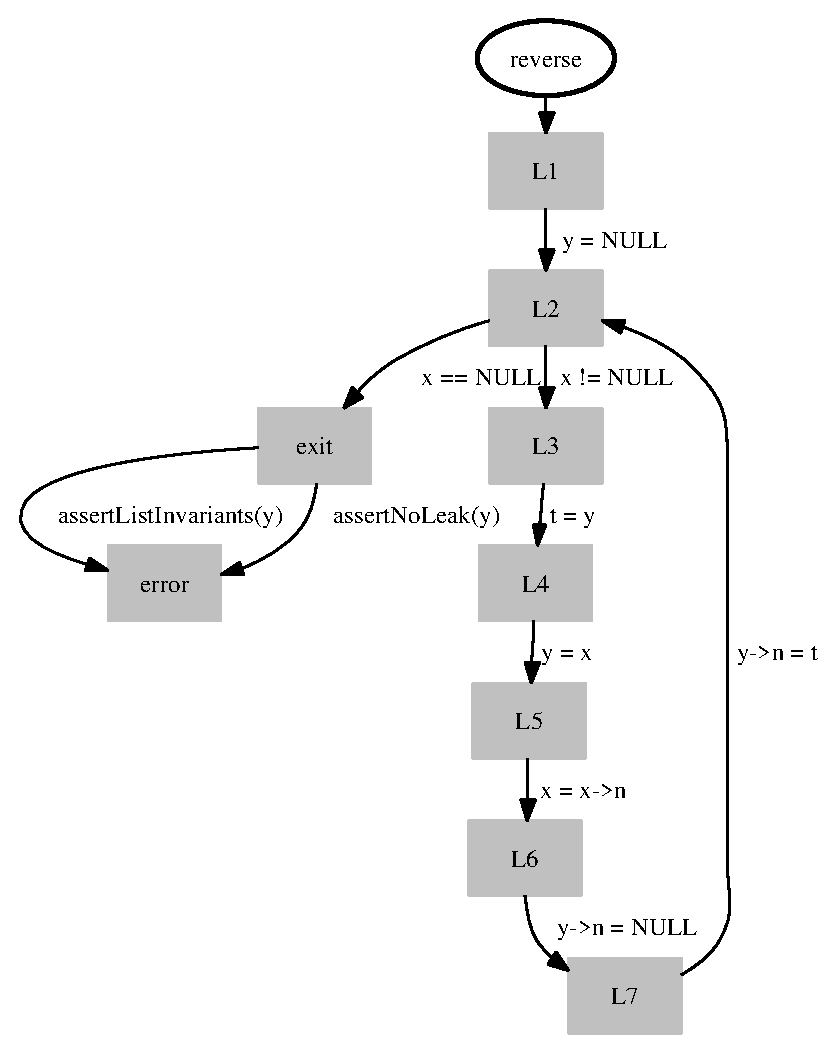
\epsfig{file=reverse_cfg,width=2.8in,height=3.0in}
\end{minipage}
\caption{\label{Fi:ManRevCFG}The CFG part of the TVP for the reverse function
shown in \figref{Reverse} and its corresponding CFG.}
\end{figure}


The specification of the analysis including the control flow graph
of the analyzed program is given in a format called TVP (Three
Valued Program). A TVP file should end with the extension '.tvp'.
The TVP for the analysis of the reverse function is given in
Figures \ref{Fi:ManRevDecl}, \ref{Fi:ManRevActions}, and
\ref{Fi:ManRevCFG}. The syntax of a TVP file is given in
\figref{TVPSyntax} and \figref{TVPSyntax2}. The syntax is in extended BNF when A $\bowtie$
B denotes a (possibly empty) sequence of A's separated by B's.

\begin{figure}
\framebox{
\begin{tabular}{ll}
\begin{minipage}[t]{1in}
\begin{tabbing}
\param{tvp} ::= \=\param{decl}$^*$ \seperator\ \param{action}$^*$ \seperator\ \\
\>\param{cfg\_edge}$^*$ \lb\seperator \csep{\param{cfg\_node}}\rb\\
\param{decl}\ \=\+::= \tvset\ \pid\ \param{set\_expr}\\
$|$ \predicate\=\ \ppred\ {\blp\ \csep{\pvar} \brp} \param{prop}$^*$\\
$|$ \instrum\=\ \ppred\ {\blp\ \csep{\pvar}\brp}\\
\>\bassign\/\ \pformula\ \param{flags}\\
$|$ \constraint\ \pformula\ \impliesT\ \pformula\\
$|$ \foreach\ \blp \param{iterator}\brp\ \blcb\ \param{decl}$^*$ \brcb\-\\
\ppred ::= \pid \lb\ \blb\ \csep{\pid}\ \brb\ \rb\\
\param{display} ::= \blcb\csep{\param{kleene}}\brcb\\
\param{iterator} ::= \pid\ \inset\ \param{set\_expr}\\
\param{kleene} ::= \textbf{1} $|$ \textbf{0} $|$ \textbf{1/2}\\
\param{action}\ \=\+::= \action\ \pid\ \blp\ \csep{\pid}\ \brp\ \blcb\\
    \lb\tvtitle\ \param{message}\rb\\
    \lb\focus\ \blcb\ \csep{\pformula}\rb\\
    \lb\precond\ \pformula\rb\\
    (\tvmessage\ \pformula\ {\bf \deref}\ \param{message})$^*$\\
    \lb\new\  \lb \pformula \rb\\
    \lb\blcb\ \param{update}$^*$\ \brcb\rb\\
    \lb\retain\ \pformula\rb \brcb\\
    (\tvmessage\ \pformula\ {\bf \deref}\ \param{message})$^*$\-\\    
\param{message}\ ::= (\param{quoted\_string}$|$\ppred)$\bowtie$\textbf{+}\\
\param{set\_expr}\ \=\+::= \param{set\_name}
$|$ \blcb\ \csep{\pid}\ \brcb\\
$|$ \param{set\_expr} \textbf{-} \param{set\_expr}\\
$|$ \param{set\_expr} \textbf{+} \param{set\_expr}\-\\
\param{update} ::=\=\ \ppred\ \blp\ \csep{\pvar}\ \brp\ \textbf{=} \pformula\\
\>$|$ \foreach\ \blp \param{iterator}\brp\ \blcb\ \param{update}$^*$ \brcb\\
\param{cfg\_edge} ::=\=\ \param{cfg\_node}\\
\>\pid\ \blp\ \csep{\pid}\ \brp\ \param{cfg\_node}\\
\end{tabbing}
\end{minipage}
&
\begin{minipage}[t]{1in}
\begin{tabbing}
// TVP file\\
\\
// Set declaration\\
// Core predicate\\
// Instrumentation predicate\\
\\
// Consistency rule\\
// For each id in the iterator\\
// Predicate name\\
// Predicate's flags\\
// Set iterator\\
// Functional dependencies\\
// Atomic values\\
// Action declaration\\
// Action title\\
// Focus formulae\\
// Precondition\\
// Report pre messages\\
// New individual(s)\\
// Update formulae\\
// Retain formula\\
// Report post messages\\
// Message for user\\
// Set definition\\
// Set difference\\
// Set union\\
// Update formula\\
// For each id in the iterator\\
// CFG edge\\
\end{tabbing}
\end{minipage}
\end{tabular}
}
\caption{\label{Fi:TVPSyntax}The syntax of a TVP file, part 1.}
\end{figure}

\begin{figure}
\framebox{
\begin{tabular}{ll}
\begin{minipage}[t]{1in}
\begin{tabbing}
\pformula\ \=\+::= \pformula\ \band\ \pformula\\
$|$ \pformula\ \bor\ \pformula\\
$|$ \pformula\ {\bf \deref} \pformula\\
$|$ \pformula\ {\bf {\tt <->}} \pformula\\
$|$ \bnot\pformula\\
$|$ \blp\pformula\=\ \textbf{?} \pformula\ \textbf{:} \pformula\brp\\
$|$ \var\ \beq\ \var\\
$|$ \var\ \bneq\ \var\\
$|$ \textbf{A}\nvars \pformula\\
$|$ \textbf{E}\nvars \pformula\\
$|$ \ppred\nvars\\
\\
$|$ \ppred\textbf{+}\twovars\\
\\
$|$ \ppred\textbf{*}\twovars\\
\\
$|$ \textbf{TC}\= \twovars\ \\
               \> \twovars\ \pformula\\
$|$ \param{kleene}\-\\
\end{tabbing}
\end{minipage}
&
\begin{minipage}[t]{1in}
\begin{tabbing}
// logical $\land$\\
// logical $\lor$\\
// logical implication\\
// logical equivalence\\
// logical $\neg$\\
// if-then-else\\
// equality\\
// inequality\\
// $\forall v_1, v_2, \ldots, v_n$\\
// $\exists v_1, v_2, \ldots, v_n$\\
// Predicate (of arbitrary\\
// arity)\\
// Transitive closure on \\
// binary predicate\\
// Reflexive and transitive \\
// closure on binary predicate\\
// Transitive closure on a\\
// general binary formula\\
// Atomic values\\
\end{tabbing}
\end{minipage}
\end{tabular}
}
\caption{\label{Fi:TVPSyntax2}The syntax of a TVP file, part 2 --- formulae.}
\end{figure}

\subsection{Predicates}
\label{Se:Predicates}

The predicate name can be either \pid\ or
\pid\blb\pid,~\ldots,~\pid\brb.
These are ordinary names.
The intention of the \pid\blb\pid,~\ldots,~\pid\brb\ format is to denote predicates which are
parameterized by source properties such as names of fields and pointer variables.
This is especially good for instrumentation predicates.
The predicate's arity is
determined by the number of variables in parenthesis.
%(currently the names of the variables are of no consequence).
For a description of the properties that can be used in predicate
declaration see \tableref{Prop}.

%%%%%%%%%%%%%% Display flags have been moved to proprty files %%%%%%%%%%%%%%%%%%%
%The \param{display} flag controls which values of the predicate are shown in the
%graph (in DOT).  The default is \{$1$, $1/2$\} specifying that true and unknown
%values are to be shown.
%%%%%%%%%%%%%%%%%%%%%%%%%%%%%%%%%%%%%%%%%%%%%%%%%%%%%%%%%%%%%%%%%%%%%%%%%%%%%%%%%

Instrumentation predicates are declared very similarly to core
predicates.  They use the same naming mechanism and the same flag
specification.  The only difference is that for an instrumentation
predicate the user has to attach its defining formula. The
formula's free variables should match the variables given in the
parenthesis (with the exception of precondition free variables
explained later).

\begin{table}
\begin{center}
\begin{tabular}{|l|l|l|l|}
\hline\hline
{\bf Property}  & {\bf Arity} & {\bf Meaning}   & {\bf Consistency Rule}\\
\hline \unique         & unary         & true for &
p(v1) \band\ p(v2) \impliesT v1 \beq\ v2\\
                &               & at most  &
E(v1) p(v1) \band\ v1 \bneq\ v \impliesT \bnot p(v)\\
                &               & one node & \\
\hline \function       & binary        & partial &
E(v) p(v, v1) \band\ p(v, v2) \impliesT v1 \beq\ v2\\
                &               & function &
E(v) p(v1, v) \band\ v2 \bneq\ v \impliesT \bnot p(v1, v2)\\
\hline \invfunction    & binary        & inverse of &
E(v) p(v1, v) \band\ p(v2, v) \impliesT v1 \beq\ v2\\
                &               & a partial &
E(v) p(v, v2) \band\ v1 \bneq\ v \impliesT \bnot p(v1, v2)\\
                &               & function &\\
\hline \symmetric      & binary        & &
p(v1, v2) \impliesT p(v2, v1)\\
\hline \antisymmetric  & binary        & &
p(v1, v2) \band\ p(v2, v1) \impliesT v1 \beq\ v2\\
                &               & &
p(v1, v2) \band\ v1 \bneq\ v2 \impliesT \bnot p(v2, v1)\\
\hline \reflexive      & binary        & &
v1 \beq\ v2 \impliesT p(v1, v2)\\
\hline \antireflexive  & binary        & &
v1 \beq\ v2 \impliesT \bnot p(v1, v2)\\
\hline \transitive     & binary        & &
E(v2) p(v1, v2) \band\ p(v2, v3) \impliesT p(v1, v3)\\
\hline \hline
\textbf{abs}    & unary         & $p$ is an     & N/A \\
                &               & abstraction   &\\
                &               & predicate     &\\
\hline
\textbf{nonabs} & unary         & $p$ is not an & N/A \\
                &               & abstraction   &\\
                &               & predicate     &\\
\hline
%\textbf{box}    & unary         & display $p$ & N/A \\
%                &               & in a box &\\
\hline \hline
\end{tabular}
\end{center}
\caption{\label{Ta:Prop}Properties of predicate p, their meaning
and the generated consistency rules.}
\end{table}

\subsection{\label{Se:FormulaeMan}Formulae}

The formula is evaluated in the context of a three valued logical
structure using the semantics of Kleene's $3$-valued logic.
Transitive closure of a general binary formula works as follows,
the last pair of variables are the free variables of the
subformula, and the first pair of variables are the variables of
the resulting TC relation.  The formula $\varphi_{cond} ?
\varphi_{true} : \varphi_{false}$ is an if-then-else formula. If
$\varphi_{cond}$ evaluates to true the value of the formula is
$\varphi_{true}$. If $\varphi_{cond}$ evaluates to false the value
of the formula is $\varphi_{false}$. If $\varphi_{cond}$ is
unknown then the result is the join of the values of
$\varphi_{true}$ and $\varphi_{false}$, i.e., the value of
$\varphi_{true}$ when it is equal to the value of
$\varphi_{false}$ and unknown otherwise.

\subsection{Consistency rules}

Most of the needed consistency rules for an analysis are
automatically generated from the functional properties of
predicates (see \tableref{Prop}) and from the instrumentation
predicates' defining formulae.  Sometimes it is useful to write
explicit consistency rules.  The left hand side of a consistency
rule (the body) is a general formula, the right hand side (the
head) is either an atomic formula or the negation of an atomic
formula, \impliesT stands for $\triangleright$.  Note that the
free variables of the body must match the free variables of the
head exactly.  A consistency rule state that for each assignment
to the free variables of the body that evaluate the body to $1$,
the head should also evaluate to $1$.  The action performed in
case of a consistency rule breach (i.e., the body of the
consistency rule is evaluated to $1$ and the head to $0$ or $1/2$
for a certain assignment) depends on the head of the consistency
rule as seen in \tableref{ConsAct}.
\begin{table}
\begin{center}
\begin{tabular}{|l|l|l|}
\hline \hline
\textbf{Head} & \textbf{Condition} & \textbf{Result}\\
\hline
0 & & The structure is invalid - discard.\\
\hline
1 & Never breached. & \\
\hline predicate & The value of the predicate for the &
The structure is invalid - discard.\\
          & assignment is false & \\
          & The value of the predicate for the & Coerce it to true.\\
          & assignment is unknown & \\
\hline
negated   & The value of the predicate for the & The structure is invalid - discard.\\
predicate & assignment is true & \\
          & The value of the predicate for the & Coerce it to false.\\
          & assignment is unknown & \\
\hline
variable & The two variables are assigned & The structure is invalid - discard.\\
equality         & to different nodes & \\
         & The variables are assigned to the & Coerce into a non summary node.\\
         & same node and it is a summary node & \\
\hline
variable  & The two variables are assigned & The structure is invalid - discard\\
inequality & to the same node & \\
\hline
\end{tabular}
\end{center}
\caption{\label{Ta:ConsAct}Result of a consistency rule breach
according to its head.}
\end{table}

\subsection{Actions}

The arguments of an action are predicate names\footnote{the
arguments can also include identifiers that are used to define
predicates.}  that can be used in the following formulae and will
be replaced with the actual arguments when the action is used (see
Section \ref{Se:CFGMan}). The actions section of the reverse
program is given in \figref{ManRevActions}.

\subsubsection{Specifying the title of an action with \tvtitle}
The title of the action, used when printing the action's
structures.

\subsubsection{Updating predicates}

Update formulae describe how predicates are updated as a result of
an action. If a predicate does not have an update formula then its
value before the action is retained. The formula is evaluated on
the old structure with the exception that nodes and predicates
added in the \new\ declaration are available. Note that update
clauses are not comma separated.

\subsubsection{Using preconditions for filtering with \precond} The
precondition formula is evaluated to check whether this action
should be performed.  If the formula is closed then a result of
true or unknown triggers the application of this action.  If the
formula contains free variables then the action is performed for
each assignment into these variables potentially satisfying the
formula.  The free variables can be used in the following formulae
and have the expected assignment.

\subsubsection{Focusing structures with \focus} The focus
formulae for this action. Applied before the precondition.

\subsubsection{Reporting messages with \tvmessage}
Messages that are reported to the user if the formula given is
potentially satisfied.

\subsubsection{Creating new nodes with \new}

An optional unary formula can be supplied. If no formula is
supplied then a single new node is created. If a formula is
supplied then each node potentially satisfying the formula is
duplicated, a new temporary binary predicate called $instance$ is
created matching the old node with the new node. In both cases an
unary predicated called $isNew$ is created an set true only for
the nodes created in this action. Both these predicates can be
used in the following formulae. The default value of all the
predicates when applied to the new nodes is false. If the unary
formula supplied evaluates to unknown for a certain node, the
matching new node becomes maybe active.

\subsubsection{Retaining nodes with \retain}

A mechanism for defining nodes that persist after an action. By
default, all nodes persist. This mechanism can be used to model
actions like free or even on-the fly garbage collection. An unary
formula must be supplied. Only nodes that potentially satisfy the
formula are retained. If the formulae supplied evaluates to
unknown for a certain node, it becomes maybe active instead of
being removed.

\subsection{\label{Se:CFGMan}Specifying the control flow graph}

The program to be analyzed is composed of CFG nodes with edges
connecting between them and actions to be performed on these
edges.  A flow insensitive analysis can be done by using a single
CFG node with actions on self loops.  A CFG node is declared
implicitly by the existence of incoming or outgoing CFG edges.
The action used in the CFG edge must be predefined in the actions
section.  The actual arguments passed to the action substitute the
formal arguments used in its definition.

If only a subset of the nodes should be printed the list of CFG
nodes to print should be supplied as the last section. The default
behavior is printing the structures available in each CFG node.


\subsection{Usability features}

TVP was designed to be written generically. Several constructs are
used to support this notion.

\subsubsection{Writing comments}

TVP supports C++ style comments: everything between /* and */ or
from // to the end of that line is ignored.

\subsubsection{Preprocessing}

The TVP file can be preprocessed using the standard C preprocessor
before being parsed by the system. The preprocessor enables file
inclusion (using the \#include directive), macro expansion (using
the \#define directive), and conditional evaluation (using the
\#if, \#endif, etc. directives).

\subsubsection{Sets}

Sets are a mechanism for grouping together several predicate names
to be used later in a \foreach\ clause or a composite formula. Set
operation such as union ($+$), and subtraction ($-$) can be used
to create set expressions.

\subsubsection{Foreach}

Sometimes a declaration, a focus formula or an update formula
should be repeated several times for different predicates, to
avoid code duplication TVP support the mechanism of \foreach. The
syntax is:

\noindent \begin{tabular}{l} \foreach\ \blp \pid\ \inset\
\param{set\_expr} \brp \blcb code \brcb
\end{tabular}

The code between the curly braces is duplicates once for each set
member and each time the predicate is substituted with the
appropriate set member.  Foreach can be applied to any declaration
(core predicate, instrumentation predicate, consistency rule), to
focus formulae and to update formulae in actions.

The \foreach\ mechanism can handle composite predicate names, in
this case only the identifiers within the square braces are
substituted.

\subsubsection{Composite operations}

Composite operations are a mechanism for applying a logical
operation (only \band\ and \bor\ are supported) on a set of
formulae.  This is similar to \foreach\ but can be used inside a
formula. The syntax is:

\noindent \begin{tabular}{l}
\param{op}/\{\pformula\ : \ppred\ \inset\ \param{set\_expr}\}
\end{tabular}

If the set is empty the neutral member for the operation is used
($0$ for \bor\ and $1$ for \band).  For example, the expression
\bor/\{$z$(v)~:~$z$~\inset~\{$x$,~$y$,~$t$\}~\} is expanded to
$x$(v)~\bor~$y$(v)~\bor~$t$(v).
